\documentclass[a4paper, 12pt]{article}
\usepackage{graphicx}
\usepackage{mathtools}
\usepackage{color}
\usepackage{epstopdf}
\usepackage[UTF8]{ctex}

\begin{document}
    {\huge\title{实验报告}}
    {\large\author{程传哲}}
    \date{\today}
    \maketitle
\section{学习成果}

\subsection{Shell}
\begin{enumerate}
  \item {\large echo \$SHELL} 
    \begin{itemize}
      \item 使用echo \$SHELL它去告诉系统这个脚本需要什么解释器来执行
      \begin{figure}[htbp]
        \centering
        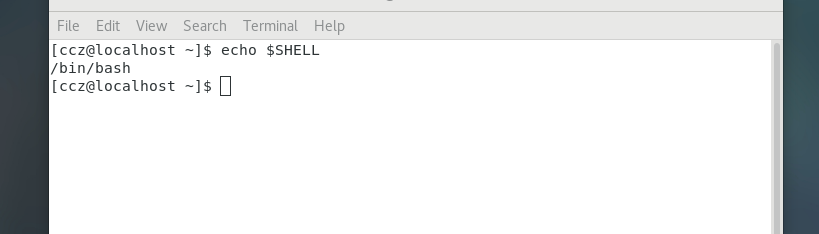
\includegraphics[scale=0.5]{1.png}
        \caption{figure title}
        \label{figure}
      \end{figure}
      \item 显示为/bash/bin的时候即shell可以使用
    \end{itemize}
  \item {\large cd tmp -- mkdir missing}
    \begin{itemize}
      \item 使用cd tmp 去切换到tmp的目录下,在使用mkdir missing 去创建一个名为missing的文件夹
      \begin{figure}[htbp]
        \centering
        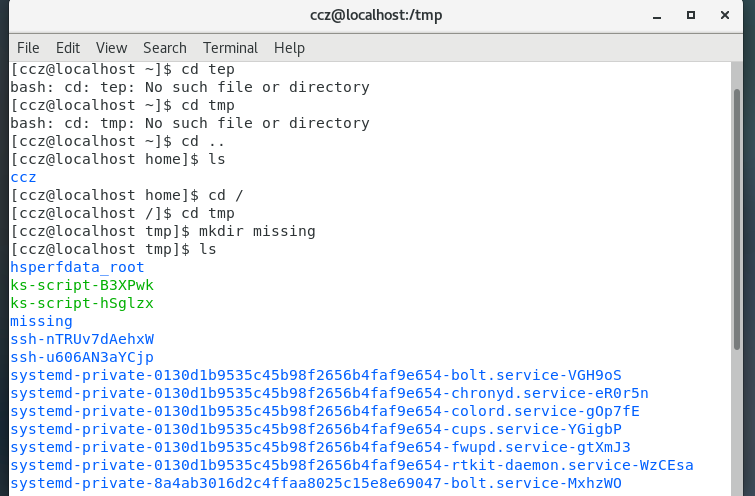
\includegraphics[scale=0.5]{2.png}
        \caption{figure title}
        \label{figure}
      \end{figure}
    \end{itemize}
  \item {\large touch semester}
    \begin{itemize}
      \item 使用semester可以在missing的目录下创建一个名为semester的文档
    \end{itemize}
  \item{\large man指令}
    \begin{itemize}
      \item man指令的作用是查看各种命令的手册,man是manual的缩写
      \item 下面是使用man touch的结果
      \begin{figure}[htbp]
        \centering
        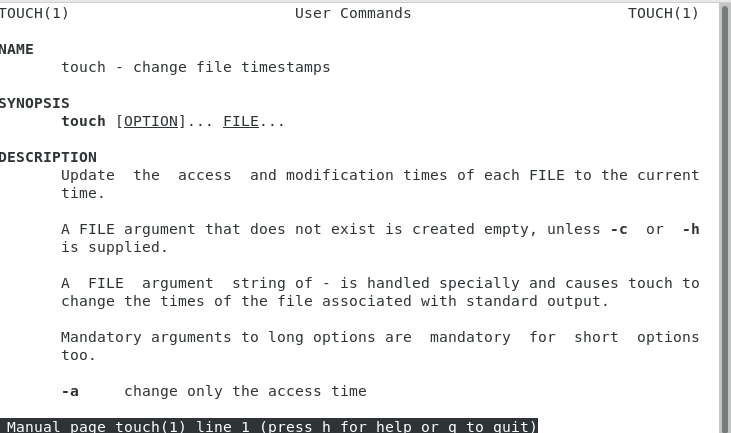
\includegraphics[scale=0.5]{4.png}
        \caption{figure title}
        \label{figure}
      \end{figure}
    \end{itemize}
  \item{\large cd ..或 cd /}
    \begin{itemize}
      \item 使用cd ..是返回至上一目录,cd /是返回至根目录
    \end{itemize}
  \item{\large pwd}
    \begin{itemize}
      \item 使用pwd是查看当前所处的文件位置
    \end{itemize}
  \item{\large ls}
    \begin{itemize}
      \item 使用ls是去查看当前文件夹下的所有文件\\
            当然ls后面可以接很多指令\\
      \begin{tabular}{|r|l|}
        \hline
        -a   & all显示所有文件及目录 (. 开头的隐藏文件也会列出)  \\
        \hline 
        -A   & 同-a但不列出 “.” (目前目录) 及 “…” (父目录)  \\
        \hline 
        -l   & 以长格式显示目录下的内容列表,包括文件的权限、链接数等  \\
        \hline 
        -d   & 仅列出目录本身,而不是列出目录内的文件数据  \\
        \hline 
        -r   & reverse,将排序结果反向输出,例如:原本文件名由小到大  \\
        \hline 
        -S   & sort by file size。根据文件大小排序,而不是文件名  \\
        \hline 
        -t   & sort by modification time,以文件修改时间排序(从最新开始排)  \\
        \hline 
        -f   & 直接列出结果,而不进行排序 (ls 默认以文件名排序)  \\
        \hline 
      \end{tabular}
    \end{itemize}
  \item{\large echo hello \textgreater  hello.txt}
    \begin{itemize}
      \item 使用echo hello \textgreater  hello.txt是将hello这个内容输入到hello.txt中
    \end{itemize}
  \item{\large cat hello.txt}
    \begin{itemize}
      \item 使用cat hello.txt可以显示出hello.txt的内容
    \end{itemize}
  \item{\large cp拷贝文件}
    \begin{itemize}
      \item 使用cp去拷贝文件有集中区分\\
      1.在当前目录下拷贝一个文件:cp \textless 现存文件名\textgreater \textless新文件名\textgreater  \\
      2.复制文件到指定目录:cp \textless现存文件名\textgreater \textless目标目录\textgreater \\
      3.复制目录及其内容:cp -r \textless现存目录名\textgreater \textless目标目录\textgreater  \\
    \end{itemize}
  \item{\large mv}
    \begin{itemize}
      \item 重命名文件
    \end{itemize}
  \item{\large pipes管道}
    \begin{itemize}
      \item \textbar  操作符允许我们将一个程序的输出和另外一个程序的输入连接起来
    \end{itemize}
\end{enumerate}
\subsection{vim文本编辑器}
\begin{enumerate}
\item{\large ESC}
  \begin{itemize}
    \item 使用ESC是为了退出编辑模式切换到命令模式
  \end{itemize}
\item{\large vi/vim}
    \begin{itemize}
      \item 通过vi/vim进入命令模式
    \end{itemize}
\item{\large -i}
    \begin{itemize}
      \item 切换到输入模式,在光标当前位置开始输入文本
    \end{itemize}
\item {\large -x}
    \begin{itemize}
        \item 删除当前光标所在处的字符
    \end{itemize}
\item {\large -u}
    \begin{itemize}
        \item 撤销上一次操作
    \end{itemize}
\item {\large -:}
    \begin{itemize}
        \item 进入底线命令模式
    \end{itemize}
\item {\large -ctrl + r}
    \begin{itemize}
        \item 重做上一次撤销的操作
    \end{itemize}
\item {\large :wq}
    \begin{itemize}
        \item 保存文件并退出
    \end{itemize}
\end{enumerate}
\subsection{shell脚本}
\begin{enumerate}
\item{\large 赋值语句}
    \begin{itemize}
        \item num = 100 回车即可操作
    \end{itemize}
\item{\large 打印语句}
    \begin{itemize}
        \item echo "num = \$num " 回车即可操作
    \end{itemize}
\item{\large 输入读取语句}
    \begin{itemize}
        \item read num 回车即可操作
        \item read -p "请输入num的值 " num 其中加入-p可以同时显示与读取
    \end{itemize}
\item{\large 只读变量}
    \begin{itemize}
        \item readonly num = 10回车即可操作 后续将无法通过赋值语句改变num的量
    \end{itemize}
\end{enumerate}
\section{Github链接}


\section{学习感悟}
    在本次的系统工具开发实践课中我受益颇多,在深入学习Shell与Vim的过程中,我经历了从初识的困惑到逐渐熟练运用的转变,这一过程不仅提升了我的技术能力,也让我对编程和命令行操作有了更深的理解和感悟,在学习shell中逐渐的了解了各个指令的用处以及shell脚本的使用,在vim的学习中学会了如何去使用vim键盘以及编写程序,这次的课程使我收益匪浅,也会继续在系统操作中继续学习下去
\end{document} 